\chapter{Theorie}
\section{Das Neuron}
Ein grundlegender Bestandteil des menschlichen Gehirns ist das Neuron. Bereits ein kleiner Ausschnitt in der Größe eines Reiskorns enthält über 10000 Neuronen, wobei jedes Neuron durchschnittlich 6000 Verbindungen mit anderen Neuronen bildet. Dieses biologische Netzwerk ermöglicht dem Menschen, die Welt um ihn herum zu erleben. Das Ziel in diesem Abschnitt ist es, diese natürliche Struktur zu nutzen, um maschinelle Lernmodelle zu entwickeln, die Probleme auf analoge Weise lösen. Hierbei ist es nicht notwendig zu wissen wie das biologische Neuron funktioniert, noch wie ein ein Netzwerk aus biologischen Neuronen arbeitet. Stattdessen wird eine mathematische Abstraktion eines Neurons formuliert, welches die Grundlage für unser neuronales Netzwerk bildet. \\
Ein Neuron mit $n$ Eingaben wird als Paar $\langle w,b \rangle$ definiert, wobei der Vektor $\mathbf{w} \in \mathbb{R}^m$ den Gewichtungsvektor und $b \in \mathbb{R}$ die Vorbelastung repräsentieren. Konzeptionell gesehen, ist das Neuron eine Funktion $p$, welche den Eingabevektor $\mathbf{x} \in \mathbb{R}^m$ auf das Intervall $[0,1]$ abbildet. Diese Funktion ist definiert als \\[0.2cm]
\hspace*{1.3cm}
$
\begin{array}[t]{lclll}
	p(\mathbf{x};\mathbf{w},b) := a(\mathbf{x}\cdot\mathbf{w}+b),
\end{array}
$
\\[0.2cm]
wobei $a$ als die sogenannte Aktivierungsfunktion bezeichnet wird (siehe Abb. \ref{fig:perceptron}).
\begin{figure}[hbt]
	\centering
	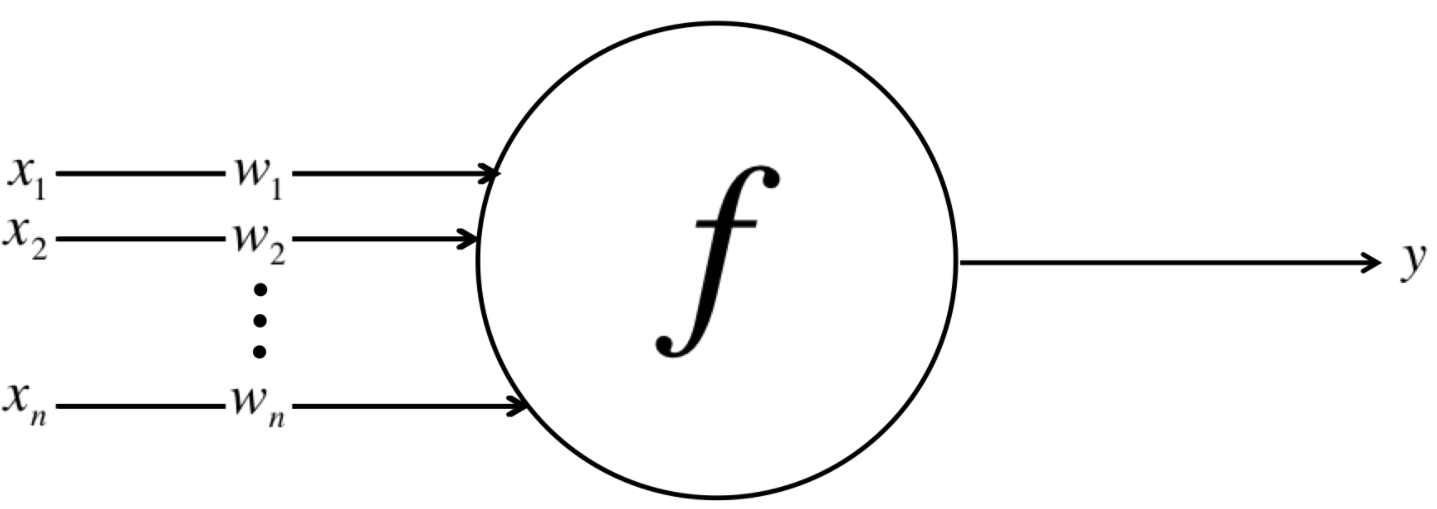
\includegraphics[scale=0.25]{Bilder/sigmoid_neuron}
	\caption{Neuron mit Eingabevektor $\mathbf{x}$, Gewichtungsvektor $\mathbf{w}$ und Ausgabe $y$.} 
	\label{fig:perceptron} 
\end{figure}

\noindent
In dieser Arbeit wird die Sigmoid-Funktion für die Aktivierung eines Neurons verwendet. Die Sigmoid-Funktion $S:\mathbb{R} \rightarrow [0,1]$ ist definiert als \\[0.2cm]
\hspace*{1.3cm}
$
\begin{array}[t]{lclll}
	S(t) := \frac{1}{1+\exp(-t)}.
\end{array}
$
\\[0.2cm]
Fällt die Betrachtung auf die Definition der Sigmoid-Funktion, lassen sich auf Basis der folgenden Überlegungen \\[0.2cm]
\hspace*{1.3cm}
$\ds\lim\limits_{x\rightarrow
-\infty} \exp(-x) = \infty$, \quad 
$\ds\lim\limits_{x\rightarrow+\infty} \exp(-x) = 0$, \quad and \quad
$\ds\lim\limits_{x\rightarrow\infty} \frac{1}{x} = 0$, 
\\[0.2cm]
die folgenden Eigenschaften ableiten: \\[0.2cm]
\hspace*{1.3cm}
$\ds \lim_{t\rightarrow-\infty} S(t) = 0$ \quad and \quad
$\ds \lim_{t\rightarrow+\infty} S(t) = 1$.
\\[0.2cm]
Die Sigmoid-Funktion $S$ konvergiert somit bei der Grenzwertbetrachtung gegen 0 bzw. 1. Eine weitere Eigenschaft der Sigmoid-Funktion besteht in deren Symmetrie (siehe Abb. \ref{fig:sigmoid_plot}). 
\begin{figure}[hbt]
	\centering
	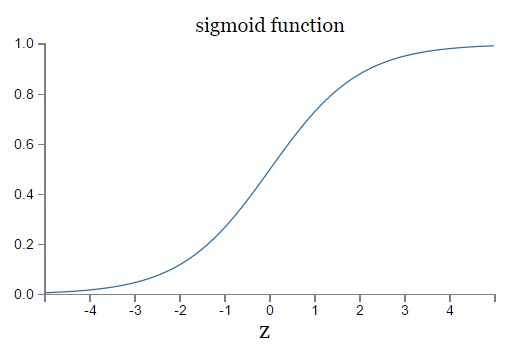
\includegraphics[scale=0.7]{Bilder/sigmoid_plot}
	\caption{Die Sigmoid-Funktion.} 
	\label{fig:sigmoid_plot} 
\end{figure}

\noindent
Bei einer Verschiebung der Funktion um $\frac{1}{2}$, liegt eine zentral symmetrische Funktion vor. \\[0.2cm]
\hspace*{1.3cm}
$S(-t)-\frac{1}{2}=-\left(S(t)-\frac{1}{2}\right)$.
\\[0.2cm]
Die Addition von $\frac{1}{2}$ auf beiden Seiten der Gleichung liefert \\[0.2cm]
\hspace*{1.3cm}
$S(-t)=1-S(t)$.
\\[0.2cm]
Fällt die Betrachtung zurück auf auf die Funktion $p$ zur Beschreibung des Neurons, liefert die Indexnotation die folgende Schreibweise. Mit \\[0.2cm]
\hspace*{1.3cm}
$\mathbf{w}=\langle w_1,\cdots ,w_m\rangle^T$
\\[0.2cm]
für den Gewichtungsvektor und \\[0.2cm]
\hspace*{1.3cm}
$\mathbf{x}=\langle x_1,\cdots ,x_m\rangle^T$
\\[0.2cm]
für den Eingabevektor, ergibt sich \\[0.2cm]
\hspace*{1.3cm}
$\ds p(\mathbf{x}; \mathbf{w}, b) = S\left(\biggl(\sum\limits_{i=1}^m x_i \cdot w_i\biggr) + b\right)$.
\\[0.2cm]

\section{Neuronales Netzwerk}
Das in dieser Arbeit angewandte Netzwerk nennt sich hierbei \textit{feedforward neural network} und beschreibt ein Netzwerk aus Neuronen, deren Informationsfluss keine Schleifen durchläuft. Die Topologie des neuronalen Netzwerk ist gegeben durch eine Zahl $L \in \mathbb{N}$ und einer Liste $[m(1),\cdots ,m(L)]$ mit $L$ natürlichen Zahlen. Hierbei bezeichnet $L$ die Anzahl der Schichten im neuronalen Netzwerk und für $i \in \{2,\cdots ,L\}$ gibt der Wert von $m(i)$ die Anzahl der Neuronen der $l$-ten Schicht an. Die erste Schicht wird in diesem Modell als Eingabeschicht bezeichnet. Sie enthält im Vergleich zu anderen Schichten keine Neuronen sondern Eingabeknoten. Die letzte Schicht (mit Index $L$) wird als Ausgabeschicht bezeichnet, wohingegen alle restlichen Schichten als verborgene Schichten bezeichnet werden. Liegen dem Netzwerk mehr wie nur eine verborgene Schicht vor, so bezeichnet man dieses als \textit{deep neural network} (siehe Abb. \ref{fig:neural_network_extended}).
\begin{figure}[hbt]
	\centering
	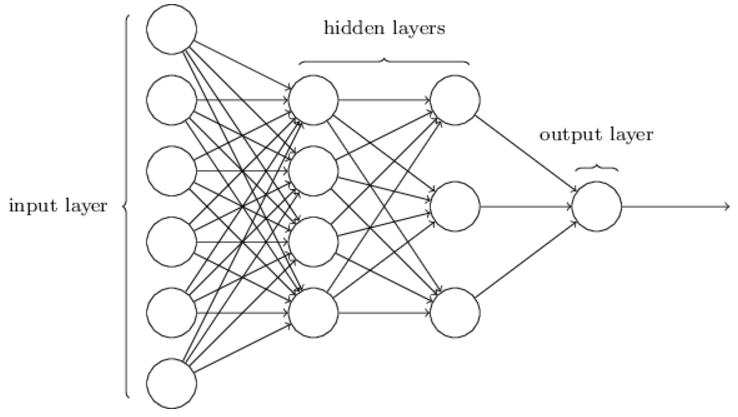
\includegraphics[scale=0.6]{Bilder/neural_network_extended}
	\caption{Aufbau des neuronalen Netzwerks hinsichtlich der einzelnen Schichten.} 
	\label{fig:neural_network_extended} 
\end{figure}

\noindent
Für die erste Schicht, die Eingabeschicht, ist die Eingabedimension definiert durch $m(1)$. Analog ist die Ausgabedimension durch $m(L)$ definiert. Jeder Knoten der $l$-ten Schicht ist zu jedem Knoten der $(l+1)$-ten Schicht über eine Gewichtung verbunden. Weiterhin ist die Gewichtung des $k$-ten Neuron der $l$-ten Schicht zu dem $j$-ten Neuron in der $(l+1)$-ten Schicht gegeben durch $w_{j,k}^{(l)}$. Alle Gewichtungen in Schicht $l$ sind über die Gewichtungsmatrix $W^{(l)}$ zusammengefasst. Die Matrix ist eine $m(l) \times m(l-1)$ Matrix mit $\ds W^{(l)} \in \mathbb{R}^{m(l) \times m(l-1)}$ und ist definiert als
\\[0.2cm]
\hspace*{1.3cm}
$\ds W^{(l)} := \bigl( w_{j,k}^{(l)} \bigr)$.
\\[0.2cm]
Das $j$-te Neuron in Schicht $l$ hat ebenfalls noch eine Vorbelastung $b_j^{(l)}$. Die Vorbelastungen der Schicht $l$ werden ebenfalls über den Vorbelastungsvektor $\mathbf{b}^{(l)}$ zusammengefasst mit
\\[0.2cm]
\hspace*{1.3cm}
$\mathbf{b}^{(l)} := \langle b_1^{(l)}, \cdots, b_{m(l)}^{(l)} \rangle^\top$.
\\[0.2cm]
Für die Aktivierungsfunktion $a_j^{(l)}$ des $j$-ten Neurons in Schicht $l$ ergibt sich hierbei die folgende rekursive Definition:
\begin{enumerate}
\item Für die erste Schicht ergibt sich
      \begin{equation}
        \label{eq:feedforward1}
       a^{(1)}_j := x_j.
      \end{equation}
      Dies bedeutet, dass der Eingabevektor $\mathbf{x}$ die Aktivierung der Eingangsknoten darstellt.
\item Für alle anderen Knoten ergibt sich
      \begin{equation}
         \label{eq:feedforward2}
         a_j^{(l)}(\mathbf{x}) := 
             S\left(\Biggl(\sum\limits_{k=1}^{m(l-1)} w_{j,k}^{(l)}\cdot a_k^{(l-1)}(\mathbf{x})\Biggr) + b_{j}^{(l)}\right) 
        \quad \mbox{$\forall l \in \{2, \cdots, L\}$}.
\end{equation}
\end{enumerate}
Der Aktivierungsvektor der $l$-ten Schicht ist somit definiert durch
\\[0.2cm]
\hspace*{1.3cm}
$\mathbf{a}^{(l)} := \langle a_1^{(l)}, \cdots, a_{m(l)}^{(l)} \rangle^\top$.
\\[0.2cm]
Des Weiteren ist die Ausgabe des neuronalen Netzwerks für eine Eingabe $\mathbf{x}$ über die Neuronen der Ausgabeschicht gegeben. Der Ausgabevektor $\mathbf{o}(\mathbf{x}) \in \mathbb{R}^{m(L)}$ ist definiert über
\\[0.2cm]
\hspace*{1.3cm}
$\mathbf{o}(\mathbf{x}) := \langle a^{(L)}_1(\mathbf{x}), \cdots, a^{(L)}_{m(L)}(\mathbf{x}) \rangle^\top = \mathbf{a}^{(L)}(\mathbf{x})$.
\\[0.2cm]
Mit den zuvor definierten Gleichungen \ref{eq:feedforward1} und \ref{eq:feedforward2} kann nun betrachtet werden, wie Informationen durch Netzwerk verbreitet werden (\textbf{feedforwarded}).
\begin{enumerate}
\item Zu Beginn ist der Eingabevektor $\mathbf{x}$ gegeben und gespeichert in der Eingabeschicht des neuronalen Netzwerks: 
      \\[0.2cm]
      \hspace*{1.3cm}
      $\mathbf{a}^{(1)}(\mathbf{x}) := \mathbf{x}$.
\item Die erste Schicht von Neuronen, welche die zweite Schicht mit Knoten darstellt, wird aktiviert und berechnet über den Aktivierungsvektor $\mathbf{a}^{(2)}$ nach der Formel
      \\[0.2cm]
      \hspace*{1.3cm}
      $\mathbf{a}^{(2)}(\mathbf{x}) := S\bigl(W^{(2)} \cdot \mathbf{a}^{(1)}(\mathbf{x}) + \mathbf{b}^{(2)}\bigr) = 
                                        S\bigl(W^{(2)} \cdot \mathbf{x} + \mathbf{b}^{(2)}\bigr)
      $.
\item Die zweite Schicht von Neuronen, welche die dritte Schicht mit Knoten darstellt, wird aktiviert und berechnet über den Aktivierungsvektor $\mathbf{a}^{(3)}$ nach der Formel
      \\[0.2cm]
      \hspace*{1.3cm}
      $\mathbf{a}^{(3)}(\mathbf{x}) := S\bigl(W^{(3)} \cdot \mathbf{a}^{(2)}(\mathbf{x}) + \mathbf{b}^{(3)}\bigr)
                          = S\Bigl(W^{(3)} \cdot S\bigl(W^{(2)} \cdot \mathbf{x} + \mathbf{b}^{(2)}\bigr) + \mathbf{b}^{(3)}\Bigr)
        $
\item Dies wird solange weitergeführt bis die Ausgabeschicht erreicht wird und die Ausgabe
      \\[0.2cm]
      \hspace*{1.3cm}
      $\mathbf{o}(\mathbf{x}) := \mathbf{a}^{(L)}(\mathbf{x})$
      \\[0.2cm]
      berechnet wurde. 
\end{enumerate}
In der folgenden Betrachtung wird angenommen, dass dem neuronalen Netzwerk $n$ Trainingsdaten mit
\\[0.2cm]
\hspace*{1.3cm}
$\langle \mathbf{x}^{(i)}, \mathbf{y}^{(i)} \rangle$ \quad for $i=1,\cdots,n$ 
\\[0.2cm]
vorliegen, sodass 
\\[0.2cm]
\hspace*{1.3cm}
$\mathbf{x}^{(i)} \in \mathbb{R}^{(1)}$ und $\mathbf{y}^{(i)} \in \mathbb{R}^{m(L)}$.
\\[0.2cm]
Das Ziel ist eine Belegung der Gewichtungsmatrix $W^{(l)}$ und dem Vorbelastungsvektor $b^{(l)}$ zu finden, damit
\\[0.2cm]
\hspace*{1.3cm}
$\mathbf{o}\bigl(\mathbf{x}^{(i)}\bigr) = \mathbf{y}^{(i)}$ \quad for all $i \in \{1,\cdots,n\}$.
\\[0.2cm]
In der Regel wird es nicht möglich sein die Gleichungen für alle $i \in \{ 1, \cdots ,n \}$ zu erfüllen, weshalb es gilt den Fehler zu minimieren. An dieser Stelle fällt die Betrachtung auf die quadratische Fehlerkostenfunktion C, die definiert ist als
\\[0.2cm]
\hspace*{1.3cm}
$\ds C\Bigr(W^{(2)}, \cdots, W^{(L)}, \mathbf{b}^{(2)}, \cdots, \mathbf{b}^{(L)};
     \mathbf{x}^{(1)}, \mathbf{y}^{(1)}, \cdots, \mathbf{x}^{(n)},\mathbf{y}^{(n)} \Bigr) := 
 \frac{1}{2 \cdot n} \cdot \sum\limits_{i=1}^n \Bigl(\mathbf{o}\bigl(\mathbf{x}^{(i)}\bigr) - \mathbf{y}^{(i)}\Bigr)^2
$.
\\[0.2cm]
An dieser Stelle ist zu berücksichtigen, dass die Kostenfunktion hinsichtlich der Trainingsdaten $\langle \mathbf{x}^{(i)},\mathbf{y}^{(i)} \rangle$ additiv ist. Eine Vereinfachung der Notation kann vorgenommen, wenn die Betrachtung bei der Kostenfunktion auf ein Trainingsbeispiel $\langle \mathbf{x},\mathbf{y} \rangle$ fällt. Dazu wird
\\[0.2cm]
\hspace*{1.3cm}
$\ds C_{\mathbf{x}, \mathbf{y}}\Bigr(W^{(2)}, \cdots, W^{(L)}, \mathbf{b}^{(2)}, \cdots, \mathbf{b}^{(L)}\Bigr) := 
 \frac{1}{2} \cdot \Bigl(\mathbf{a}^{(L)}\bigl(\mathbf{x}\bigr) - \mathbf{y}\Bigr)^2
$
\\[0.2cm]
definiert. Weiterhin ergibt sich für die allgemeine Kostenfunktion
\\[0.2cm]
$\ds C\Bigr(W^{(2)}, \cdots, W^{(L)}, \mathbf{b}^{(2)}, \cdots, \mathbf{b}^{(L)};
     \mathbf{x}^{(1)}, \mathbf{y}^{(1)}, \cdots, \mathbf{x}^{(n)},\mathbf{y}^{(n)} \Bigr) := 
 \frac{1}{n} \cdot \sum\limits_{i=1}^n C_{\mathbf{x^{(i)}}, \mathbf{y}^{(i)}}\Bigr(W^{(2)}, \cdots W^{(L)}, \mathbf{b}^{(2)}, \cdots, \mathbf{b}^{(L)}\Bigr) 
$.
\\[0.2cm]
Für den weiteren Verlauf dieser Arbeit die Notation $C_{\mathbf{x}, \mathbf{y}}$ für den Ausdruck
\\[0.2cm]
\hspace*{1.3cm}
$\ds C_{\mathbf{x}, \mathbf{y}}\Bigr(W^{(2)}, \cdots, W^{(L)}, \mathbf{b}^{(2)}, \cdots, \mathbf{b}^{(L)}\Bigr)$
\\[0.2cm]
eingeführt.


\section{Backpropagation}
Der Backpropagation-Algorithmus ist das meist genutzte neuronale Modell. Grund ist die universelle Einsetzbarkeit für beliebige Approximationsaufgaben im Hinblick auf die effiziente Berechnung der partiellen Ableitung der Kostenfunktion $C$ nach der Gewichtung $w_{j,k}^{(l)}$ und der Vorbelastungen $b_j^{(l)}$. Ziel des Algorithmus ist die Minimierung der Abweichung zwischen erwartetem Ausgabewert und dem durch das neuronale Netzwerk ermitteltem Wert. Hierzu wird in dem folgenden Kapitel das Werkzeug für dessen Berechnung gegeben. \\

%http://download.springer.com/static/pdf/442/chp%253A10.1007%252F978-3-658-13549-2_9.pdf?originUrl=http%3A%2F%2Flink.springer.com%2Fchapter%2F10.1007%2F978-3-658-13549-2_9&token2=exp=1494935592~acl=%2Fstatic%2Fpdf%2F442%2Fchp%25253A10.1007%25252F978-3-658-13549-2_9.pdf%3ForiginUrl%3Dhttp%253A%252F%252Flink.springer.com%252Fchapter%252F10.1007%252F978-3-658-13549-2_9*~hmac=259dec5f34cd0b3359f1147eaa21cf718b54fe7ffd8f04118d36cf45e9be83ef

\noindent
Für die Backpropagation-Gleichungen werden zunächst Hilfsgrößen definiert, damit. \\
Die Definition von $z_j^{(l)}$, soll die Eingabe der Aktivierungsfunktion $S$ des $j$-ten Neuron der $l$-ten Schicht darstellen:
\\[0.2cm]
\hspace*{1.3cm}
$\ds z_j^{(l)} := \left(\sum\limits_{k=1}^{m(l-1)}  w_{j,k}^{(l)} \cdot a_k^{(l-1)}\right) + b_j^{(l)}$
\quad $\forall j \in \{1, \cdots, m(l)\}$ und $\forall l \in \{2,\cdots,L\}$.
\\[0.2cm]
Im Wesentlichen ist $z_j^{(l)}$ die Eingabe der Sigmoid-Funktion, damit die Aktivierung $a_j^{(l)}$ mit
\\[0.2cm]
\hspace*{1.3cm}
$a_j^{(l)} = S(z_j^{(l)})$.
\\[0.2cm]
berechnet werden kann. Angenommen im $j$-ten Neuron der $l$-ten Schicht erfahren die Berechnungen eine zusätzliche Änderung $\Delta z_j^{(l)}$.  Dadurch erfährt die Aktivierung des nachgelagerten Neuron den folgenden Zusatz: 
\\[0.2cm]
\hspace*{1.3cm}
$a_j^{(l)}=S(z_j^{(l)}+\Delta z_j^{(l)})$.
\\[0.2cm]
Diese Änderungen wird durch das neuronale Netzwerk weitergeleitet und kann entsprechende Auswirkungen auf die korrekte Bestimmung der Eingaben haben. Damit Fehler vermieder werden empfiehlt sich im Hinblick auf die partielle Ableitung der Kostenfunktion $C_{\mathbf{x},\mathbf{y}}$ nach der Gewichtung $w_{j,k}^{(l)}$ und den Vorbelastungen $b_j^{(l)}$ zuerst die Berechnung der partiellen Ableitung von $C_{\mathbf{x},\mathbf{y}}$ nach $z_j^{(l)}$ durchzuführen. Hierzu sei folgende Definition gegeben:
\\[0.2cm]
\hspace*{1.3cm}
$\ds\varepsilon_j^{(l)} := \frac{\partial C_{\mathbf{x}, \mathbf{y}}}{\partial z_j^{(l)}}$ \quad $\forall j \in \{1, \cdots, m(l)\}$ und $\forall l \in \{2,\cdots, L\}$,
\\[0.2cm]
An dieser Stelle ist zu berücksichtigen, dass die partielle Ableitung $\ds\varepsilon_j^{(l)}$ abhängig von $\mathbf{x}$ und $\mathbf{y}$ ist. Weiterhin werden die Größen $\ds\varepsilon_j^{(l)}$ in dem Vektor
\\[0.2cm]
\hspace*{1.3cm}
$\boldsymbol{\varepsilon}^{(l)} := \left(
  \begin{array}[c]{c}
    \varepsilon_1^{(l)}      \\
    \vdots             \\
    \varepsilon_{m(l)}^{(l)}  
  \end{array}
  \right)
$.
\\[0.2cm]
zusammengefasst und als \textit{Fehler in Schicht l} bezeichnet.

\noindent
Mit den definierten Hilfsgrößen ist es nun möglich die vier Gleichung für die Backpropagation zu beschreiben. 
 
\begin{enumerate}
\item Die erste Gleichungen berechnet $\varepsilon^{(L)}_j$ für $l=L$, wobei $S'(x)$ die Ableitung der Sigmoid-Funktion bezeichnet. Mit dieser Gleichung wir der Fehler in der Ausgabeschicht berechnet.
\begin{equation}
	\label{eq:BP1}
	\varepsilon^{(L)}_j = (a_j^{(L)} - y_j) \cdot S'\bigl(z_j^{(L)}\bigr)
	\quad \mbox{$\forall j \in \{1, \cdots, m(L)\}$}.
\end{equation}
Die Gleichung \ref{eq:BP1} kann auch als vektorisierte Schreibweise mittels dem Hardamard-Produkt angegeben werden. Hierfür ergibt sich:
\begin{equation}
  \label{eq:BP1s}
\boldsymbol{\varepsilon}^{(L)} = (\mathbf{a}^{(L)} - \mathbf{y}) \odot S'\bigl(\mathbf{z}^{(L)}\bigr)  
\end{equation}
    
\item Die zweite Gleichung berechnet $\varepsilon^{(L)}_j$ für alle $l<L$. Der Fehler $\boldsymbol{\varepsilon}^{(l+1)}$ von Schicht $l+1$ fließt hierbei in die Berechnung von $\boldsymbol{\varepsilon}^{(l)}$ ein.
\begin{equation}
	\label{eq:BP2}
	\varepsilon^{(l)}_j = \sum\limits_{i=1}^{m(l+1)} w_{i,j}^{(l+1)} \cdot 			\varepsilon^{(l+1)}_i \cdot S'\bigl(z^{(l)}_j\bigr) \quad \mbox{ $\forall j \in \{1, \cdots, m(l)\}$ und $\forall l \in \{2, \cdots, L-1\}$}
\end{equation}
Auch diese Gleichung kann in der vektorisierten Schreibweise angegeben werden:
\begin{equation}
  \label{eq:BP2v}
  \boldsymbol{\varepsilon}^{(l)} = \Bigl(\bigl(W^{(l+1)}\bigr)^\top \cdot \boldsymbol{\varepsilon}^{(l+1)}\Bigr) \odot
  S'\bigl(z^{(l)}\bigr) \quad \mbox{$\forall l \in \{2, \cdots, L-1\}$}.
\end{equation}

\item Die nächste Gleichung ist durch die partielle Ableitung von $C_{\mathbf{x},\mathbf{y}}$ nach der Vorbelastung $b_j^{(l)}$ des $j$-ten Neuron in Schicht $l$ gegeben. Diese Gleichung gibt somit die Änderungsrate der Kosten hinsichtlich der Vorbelastungen an.
\begin{equation}
  \label{eq:BP3}
  \frac{\partial C_{\mathbf{x}, \mathbf{y}}}{b_j^{(l)}} = \varepsilon_j^{(l)}
  \quad \mbox{$\forall j \in \{1,\cdots,m(l)\}$ und $\forall l \in \{2, \cdots,l\}$}
\end{equation}
Die vektorisierte Schreibweise nimmt hierbei die folgende Form an:
\begin{equation}
  \label{eq:BP3v}
  \nabla_{\mathbf{b}^{(l)}} C_{\mathbf{x}, \mathbf{y}} = \boldsymbol{\varepsilon}^{(l)}
  \quad \mbox{$\forall l \in \{2, \cdots,l\}$}
\end{equation}
Mit $\nabla_{\mathbf{b}^{(l)}}$ wird in dieser Arbeit der Gradient von $C_{\mathbf{x},\mathbf{y}}$ im Hinblick auf $b^{(l)}$ bezeichnet. 

\item Die letzte Gleichung ist durch die partielle Ableitung von $C_{\mathbf{x},\mathbf{y}}$ nach der Gewichtung $w_{j,k}^{(l)}$ gegeben. Diese Gleichung gibt somit die Änderungsrate der Kosten hinsichtlich der Gewichtungen an.
\begin{equation}
  \label{eq:BP4}
  \frac{\partial C_{\mathbf{x}, \mathbf{y}}}{\partial w_{j,k}^{(l)}} = a_k^{(l-1)} \cdot \varepsilon_j^{(l)}
  \quad \mbox{$\forall j \in \{1,\cdots,m(l)\}$, $\forall k \in \{1,\cdots,m(l-1)\}$, $\forall l \in \{2, \cdots,l\}$}
\end{equation}
Die vektorisierte Schreibweise liefert auch in diesem Fall die folgende Form:
\begin{equation}
  \label{eq:BP4v}
  \nabla_{W^{(l)}} C_{\mathbf{x}, \mathbf{y}} = \boldsymbol{\varepsilon}^{(l)} \cdot \bigl(\mathbf{a}^{(l-1)}\bigr)^\top
  \quad \mbox{$\forall l \in \{2, \cdots,l\}$}
\end{equation}
Der Ausdruck $\boldsymbol{\varepsilon}^{(l)} \cdot \bigl(\mathbf{a}^{(l-1)}\bigr)^\top$ bezeichnet hierbei die Matrixmultiplikation zwischen dem Spaltenvektor $\boldsymbol{\varepsilon}^{(l)}$ als $m(l) \times 1$ Matrix und dem Reihenvektor $\bigl(\mathbf{a}^{(l-1)}\bigr)^\top$ als $1 \times m(l-1)$ Matrix.
\end{enumerate}

\noindent
Bei Anbetracht der Gleichungen \ref{eq:BP3} und \ref{eq:BP4v} wird nun ersichtlich, weshalb die Einführung des Vektors $\boldsymbol{\varepsilon}^{(l)}$ von Vorteil war. Dieser Vektor ermöglicht die partielle Ableitung nach den Gewichtungen sowie den Vorbelastungen für die Kostenfunktion. Ebenfalls wurde die vektorisierte Schreibweise für die einzelnen Gleichungen in diesem Abschnitt aus Effizienzgründen für die spätere Implementierung eingeführt. Dies liegt in der schnelleren Ausführung von Matrix-Vektor-Multiplikationen bei Interpretersprachen wie z.B. SetlX begründet. \\

\section{Stochastic Gradient Descent}
Für eine zuverlässige Klassifizierung der Eingaben wird eine Algorithmus benötigt, welcher die Bestimmung von Gewichtungen und Vorbelastungen bestmöglich gewährleistet. Hierzu wird in dieser Arbeit auf die Methode des \textit{Stochastic Gradient Descent} zurückgegriffen. Im Bereich des maschinellen Lernen ist es notwendig das Minimum oder Maximum einer Funktion \\[0.2cm]
\hspace*{1.3cm}
$f:\mathbb{R}^n \rightarrow \mathbb{R}$.
\\[0.2cm]
zu ermitteln. Die im vorangegangenen Kapitel vorgestellten Gleichungen der Backpropagation beschreiben den Gradienten der Kostenfunktion für eine einzelnes Trainingsbeispiel $\langle\mathbf{x}, \mathbf{y}\rangle$. Besteh die Absicht unser neuronales Netzwerk zu trainieren, müssen alle Trainingsdaten berücksichtigt werden. Für $n$ Trainingsdaten 
\\[0.2cm]
\hspace*{1.3cm}
$\langle\mathbf{x}^{(1)}, \mathbf{y}^{(1)}\rangle$,
$\langle\mathbf{x}^{(2)}, \mathbf{y}^{(2)}\rangle$,
$\cdots$,
$\langle\mathbf{x}^{(n)}, \mathbf{y}^{(n)}\rangle$,
\\[0.2cm]
wurde die quadratische Fehlerkostenfunktion bereits wie folgt definiert: 
\\[0.2cm]
\hspace*{1.3cm}
$\ds C\Bigr(W^{(2)}, \cdots, W^{(L)}, \mathbf{b}^{(2)}, \cdots, \mathbf{b}^{(L)};
     \mathbf{x}^{(1)}, \mathbf{y}^{(1)}, \cdots, \mathbf{x}^{(n)},\mathbf{y}^{(n)} \Bigr) := 
 \frac{1}{2 \cdot n} \cdot \sum\limits_{i=1}^n \Bigl(\mathbf{o}\bigl(\mathbf{x}^{(i)}\bigr) - \mathbf{y}^{(i)}\Bigr)^2
$.
\\[0.2cm]
Wenn die Berechnung der Gradienten für die quadratische Fehlerkostenfunktion hinsichtlich einer Gewichtungsmatrix $W^{(l)}$ oder einer Vorbelastung $b^{(l)}$ vorgenommen werden soll, müssen die Summen
\\[0.2cm]
\hspace*{1.3cm}
$\ds \frac{1}{2\cdot n} \cdot \sum\limits_{i=1}^n \frac{\partial C_{\mathbf{x}^{(i)}, \mathbf{y}^{(i)}}}{\partial w_{j,k}^{(l)}}$
\quad and \quad
$\ds \frac{1}{2\cdot n} \cdot \sum\limits_{i=1}^n \frac{\partial C_{\mathbf{x}^{(i)}, \mathbf{y}^{(i)}}}{\partial b_{j}^{(l)}}$
\\[0.2cm]
über alle Trainingsdaten für einen Iterationsschritt des \textit{Gradient Descent} berechnet werden. Dies kann mit einer großen Anzahl von Trainingdaten kostenintensive Auswirkungen haben, weshalb beim \textit{Stochastic Gradient Descent} für die Berechnung der Summen eine zufällige Teilmenge aus den Trainingsdaten für die Abschätzung herangezogen wird. Bei einer Teilmenge mit $m$ Trainingsdaten, liegt die folgende Abschätzung zugrunde:
\\[0.2cm]
$\ds \frac{1}{2\cdot n} \cdot \sum\limits_{i=1}^n \frac{\partial C_{\mathbf{x}^{(i)}, \mathbf{y}^{(i)}}}{\partial w_{j,k}^{(l)}}
 \approx
 \frac{1}{2\cdot m} \cdot \sum\limits_{i=1}^m \frac{\partial C_{\mathbf{x}^{(i)}, \mathbf{y}^{(i)}}}{\partial w_{j,k}^{(l)}}
$
\quad und \quad
$\ds \frac{1}{2\cdot n} \cdot \sum\limits_{i=1}^n \frac{\partial C_{\mathbf{x}^{(i)}, \mathbf{y}^{(i)}}}{\partial b_{j}^{(l)}}
     \approx
     \frac{1}{2\cdot m} \cdot \sum\limits_{i=1}^m \frac{\partial C_{\mathbf{x}^{(i)}, \mathbf{y}^{(i)}}}{\partial b_{j}^{(l)}}
$.
\\[0.2cm]
Die Namensgebung für diese Methode, ist durch die zufällige Trainingdatenauswahl zu erklären. Im Vergleich zur \textit{Gradient Descent} Methode, kann sie das Lernen in neuronalen Netzwerken erheblich beschleunigen, da nicht alle Trainingsdaten in den Prozess einfließen.